\documentclass[fontsize=11pt]{article}
    \usepackage{amsmath}
    \usepackage[utf8]{inputenc}
    \usepackage{graphicx}
    \usepackage[margin=0.75in]{geometry}
    \usepackage{hyperref}
    \hypersetup{
        colorlinks=true,
        urlcolor=blue,
        }

    \title{CSC111 Project Report: Mapping Wikipedia Article Structure}
    \author{Benjamin Fitzgerald, Samuel Reeder, Vedant Swamy, Raymond Zeng-Xu}
    \date{Sunday, April 2, 2023}

    \begin{document}
    \maketitle

    \section*{Introduction}

    Wikipedia is an online encyclopedia that contains more than six million English articles. It is actively maintained and expanded by tens of thousands of volunteers called "editors", who work on articles according to general guidelines. The encyclopedia is a highly popular source of knowledge: Wikipedia.org is the 6th most visited website in the world. Due to its size and importance, the organization of information on Wikipedia is of great academic interest: Wikipedia is (in some sense) a reflection of collective human knowledge. Therefore, insights into the structure of Wikipedia articles can reveal valuable information about how knowledge is organized in society, or how different categories of knowledge relate to each other. A well-known example of this is the phenomenon termed "getting to philosophy". Nearly all Wikipedia articles contain at least one \textit{hyperlink}: a word in a Wikipedia article that links to another article, (possibily itself). If the first non-italicized, non-parenthesized hyperlink in a Wikipedia article is chosen, and then the first hyperlink in that article, and so forth, it has a pretty good chance of getting to the Wikipedia article on Philosophy. Actually, more than \textit{90 percent} of Wikipedia articles will eventually lead to the philosophy article if this algorithm is performed. This phenomena occurs because it is standard practice on Wikipedia to start an article with a general description of a topic. This general description usually includes a broader category that the topic belongs to (for example, the topic "chemistry" belongs to the broader category "science"). Intuitively, philosophy is a very broad category, since it is the foundation of every area of study. So in this way, Wikipedia "reflects" how we internally categorize information, i.e. chemistry $\rightarrow$ is a subset of physics $\rightarrow$ is a subset of math $\rightarrow$ is a subset of philosophy. This raises an interesting question: what other articles have a large portion of Wikipedia link to them eventually? What other relationships can we find by exploring hyperlinks in an iterative way? On the English Wikipedia, nearly all articles are placed in specific categories: (History and events, geography and places, human activities, etc.). Each article can belong to multiple categories. Thus, each article on Wikipedia is associated with a set of categories that it belongs to. As a result, we can also ask: what is the relationship between the size of an article, its connections, and its categories? For example, is there an correlation between the size of an article (it terms of its word count) and how many categories it belongs to? This leads us to the goal of this project:

    \begin{enumerate}

    \item{\textbf{Graphically represent connections between Wikipedia articles by hyperlinks, using categories and article size.}}

    \item{\textbf{Locate "general" articles that many articles eventually hyperlink to.}}

    \item{\textbf{Draw conclusions about how knowledge on Wikipedia is organized according to article hyperlinks.}}

    \end{enumerate}

    Note: for the third goal, the way data is organized by hyperlinks is likely not the same as the \textit{article categories} mentioned above.

	\section*{Datasets}
	
	We obtained all our data from the MediaWiki API. It provides the hyperlinks going out from an article, the categories articles belong to, and the size of the articles (in terms of word count). 

\section*{Computational Overview}
    \subsection*{The \textit{DirectedGraph} Class}
    We used directed graphs to represent connectivity between Wikipedia articles and other Wikipedia articles that are directly connected by reference through hyperlinks. We preserve most of the common properties of directed graphs that are present in lectures but supplement them with additional properties and use lists as opposed to sets in some places. Each node on the graph is represented as a connected article.
    
    \subsection*{API}
    Sending a request using \textit{requests} module's \textit{.get()}, we take an article and make a call to the MediaWiki API to get all desired properties of the article. 
    \subsection*{Graph Visualization}
    Once we gather the properties of the parent article, we recursively perform the same above steps for all articles referenced as a hyperlink in the parent, until the maximum recursion depth is reached. We establish edges between the above parent article and each daughter. They are not all added simultaneously. Additionally, we surf the graph to identify whether newly added articles connect to any previous articles and establish those edges. If category filters are specified, it performs the same steps but omits articles that do not adhere to the category rules and restrict recursion through their respective hyperlinks. Importantly, networkx's \textit{spring\_layout()} uses the Fruchterman-Reingold algorithm, that minimizes the amount of overlapping edges to produce neater-looking graphs. Plotly's \textit{graph\_objects} module provides necessary functions for creating a scatter plot, allowing us to manipulate point size, color, and placement to represent node properties.
    \subsection*{Statistics.py}
The Statistics.py file contains three functions that take a DirectedGraph instance as input: The first one calculates the vertex with the most number of edges. The second one calculates the vertex with the maximum ratio of output to input edges. The third one calculates the vertex with the maximum ratio of input to output edges. If there is a tie, then all the tied vertices are returned. 
    
    \section*{Instructions}
    Simply call the \textit{main} function in \textit{main.py}. You must pass the article title, depth, and what color on the graph should indicate (either category size or article size). The function will return a graph, as well as relevant statistical data pertaining to it. The graph will inclde the passed article, as well as the hyperlinks that leave it, and the hyperlinks that leave those articles, and so forth up to the given depth. A depth of 1 returns the article itself. Be sure that the given article is a valid  English Wikipedia article title. 
    
    \section*{Changes to Project Plan}
    
    We graphed the number of categories each article belongs to instead of \textit{which} categories each article belongs to. We also only graphed a very small subset of all English Wikipedia articles (nothing close to the entire thing). 
    
    
    
    \section*{Discussion of Results}
    
    \subsection*{ 1. Graphically Represent Connections}
    Overall the graphical representation of connections is very successful. Even though only a few thousand articles can be graphed at a time, each graph nicely contains all the information we sought: the connections between articles, how many connections they have, their size (word count) and how many categories they occupy. We Did not represent \textit{which} category they occupy. We can make detailed graphs of any Wikipedia article and thousands of its neighbors. 
    
    \subsection*{ 2. Locate "General" Articles}
    The graphs and statistical data give us an idea of which articles are general. For example, below is the output of main("History", 2, True, set()). 
    
    \begin{figure}[h!]
    \begin{center}
  		\includegraphics[width=0.7\textwidth]{HistoryD2.png}
  		\caption{Output of \textit{main("History", 2, True, set())}}
  		\label{fig:}
  	\end{center}
	\end{figure}
	
	"History" has a large number of connections compared to its neighbors. So it can be reasonably assumed that "History" is a general topic, since its neighbors have fewer connections. It is plausible that, if history was a general topic, some of its neighbors would have a very large number of connections, because the neighbors of history would be connected to each other. However, this is note the case. It is still unclear which articles behave similarly to the "getting-to-philosophy" phonomenon. Thus, while we have a measurement of generality from the graph, we still do not know what pecent of the entire Wikipedia eventually hyperlinks to a specific article.
	
	
	\subsection*{3. Drawing Conclusions About how Data is Organized}
	
	
	
	\begin{figure}[h!]
    \begin{center}
  		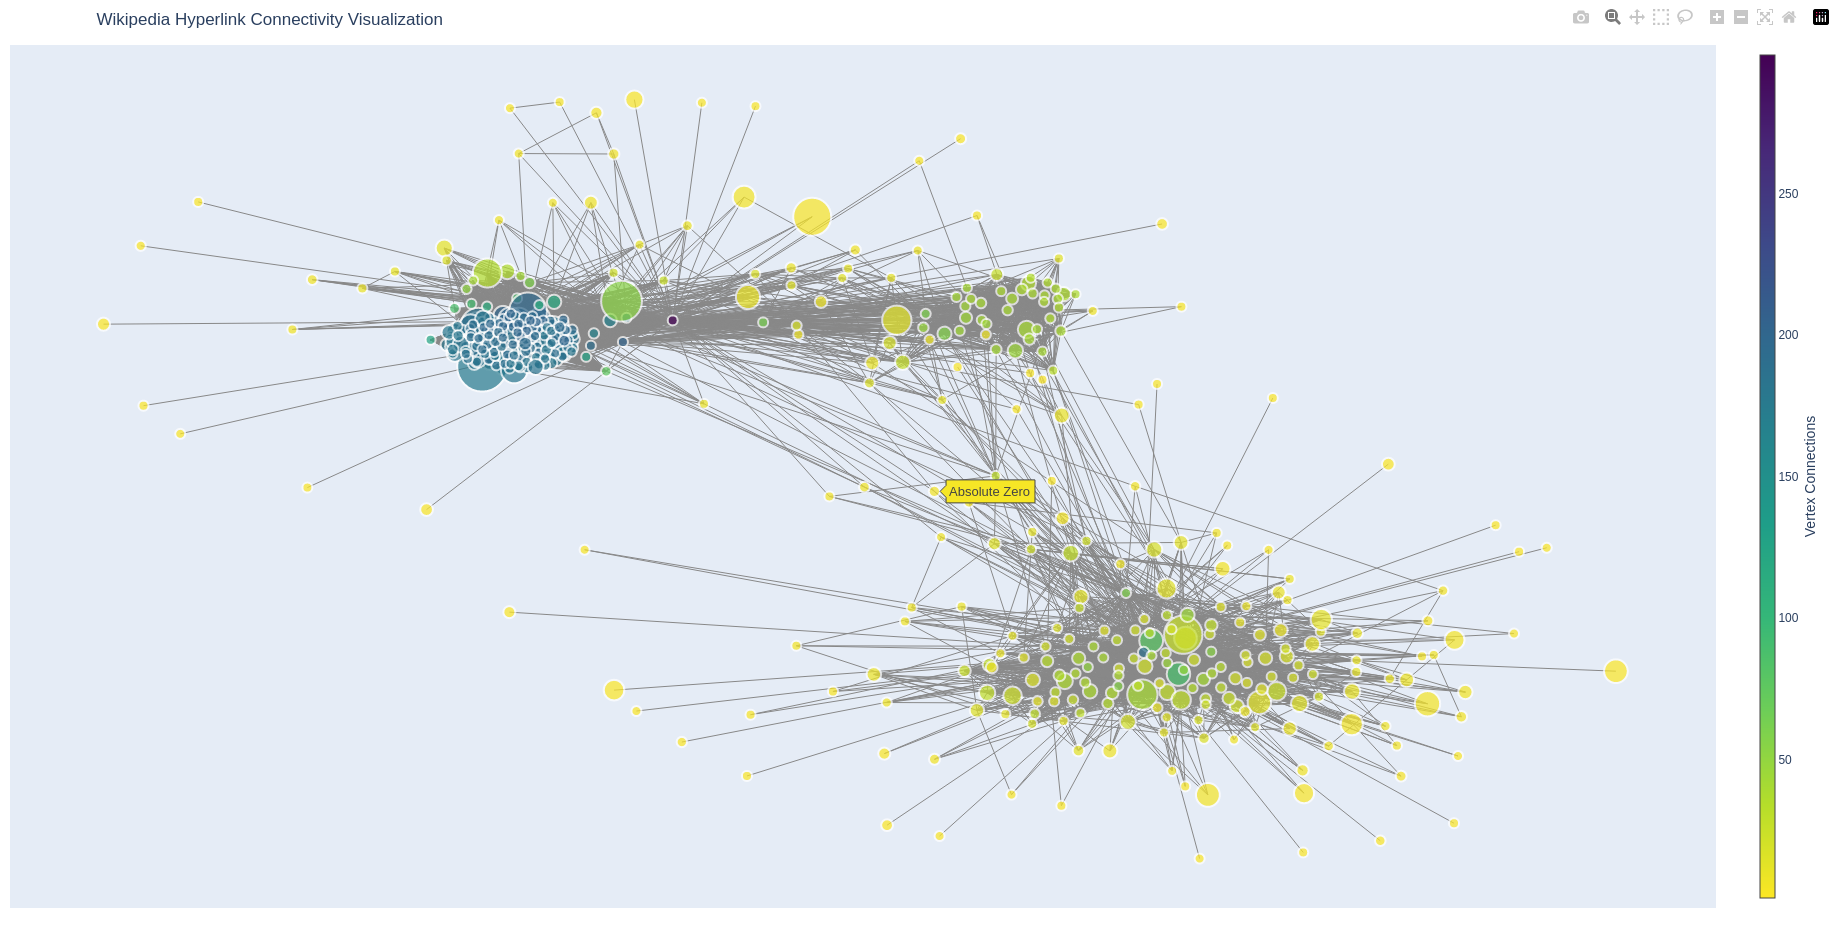
\includegraphics[width=0.7\textwidth]{AbsoluteZeroConnections.png}
  		\caption{Graph starting at "Absolute Zero" with color representing connections.}
  		\label{fig:}
  	\end{center}
	\end{figure}
	
	 \begin{figure}[h!]
    \begin{center}
  		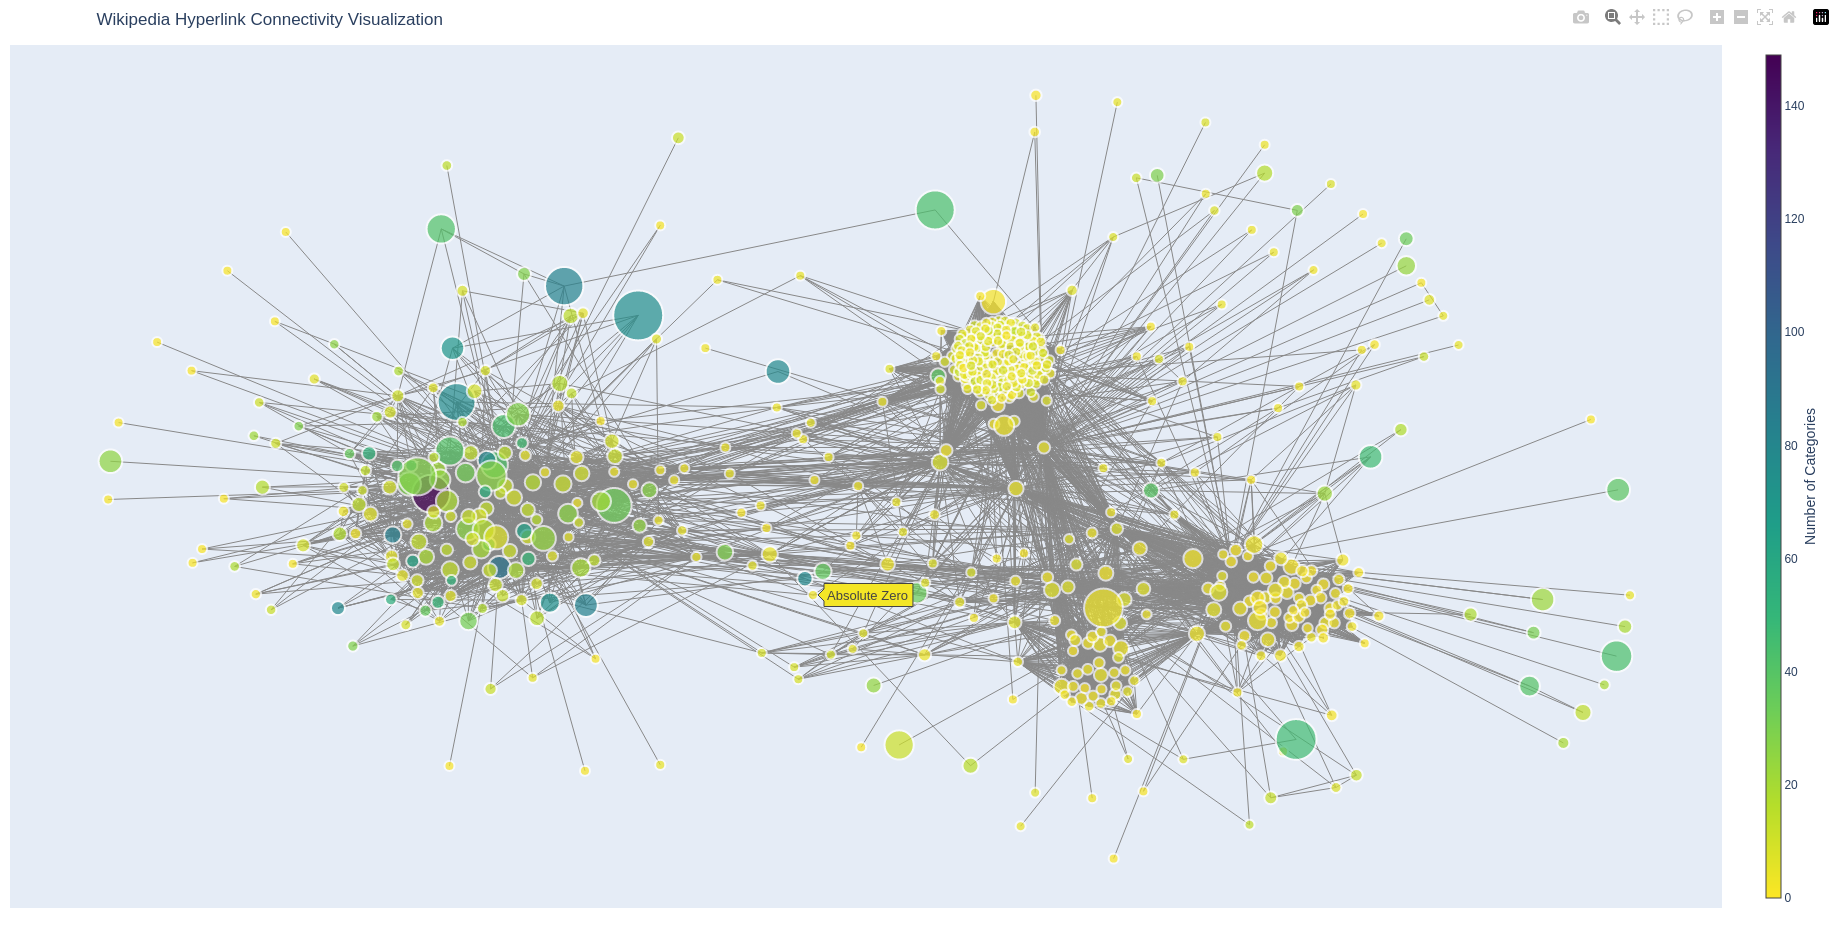
\includegraphics[width=0.7\textwidth]{AbsoluteZeroCategories.png}
  		\caption{Graph starting at "Absolute Zero" with color representing categories.}
  		\label{fig:}
  	\end{center}
	\end{figure}
	
	By looking at various graphs, we can see how article size relates to category. An interesting conclusion we can draw is that very large articles tend to be a part of a large number of categories. This makes sense, because topics that are a part of many categories simultaneously tend to be very important (for example, the article on Albert Einstein is the categories for important poeple, physics, science, etc). We can also see that articles that have a large number of categories may not necessary have a large number of nodes (for example, the "Absolute Zero" graph). The graphs of a large random sample of articles will need to be examined before any definite statistical conclusion can be drawn. We did not determine the relationship between different categories. 
	
	
\section*{Discussion}

	We were able to gather some interesting insights into the structure of Wikipedia articles, but we were unable to determine which articles most Wikipedia articles eventually link to when repeatedly traversing hyperlinks. There is likely a strong pattern between catagory size, node connections, and article size. To further our research we should call \textit{main()} on a large random sample of articles in order to work out these patterns using regression. Another possible direction of research is to use more computational resources so that the graphs include more articles and possibly even the entire English Wikipedia itself. Additionally, it should be possible to determine the relationship between different categories by filtering them using the "categories" parameter of \textit{main()}. 
	

	
    
    
    
    
    
    
    

    

   

   

    \section*{References}
    \begin{enumerate}
        \item “API:Main Page - MediaWiki.” \textit{MediaWiki}. Retrieved March 8, 2023 from
        \url{https://www.mediawiki.org/wiki/API:Main\_page}.
        \item “API:Properties - MediaWiki." \textit{MediaWiki}. \url{https://www.mediawiki.org/wiki/API:Properties}.
        \item “API:Categoryinfo - MediaWiki." \textit{MediaWiki}. Retrieved March 8, 2023 from
        \url{https://www.mediawiki.org/wiki/API:Categoryinfo}.
        \item “API:Categorymembers - MediaWiki." \textit{MediaWiki}. Retrieved March 8, 2023 from
        \url{https://www.mediawiki.org/wiki/API:Categorymembers}.
        \item “API:Allpages - MediaWiki." \textit{MediaWiki}. Retrieved March 8, 2023 from
        \url{https://www.mediawiki.org/wiki/API:Allpages}.
        \item "Getting to Philosophy." \textit{Wikipedia}. Retrieved March 8, 2023 from
        \url{https://en.wikipedia.org/wiki/Wikipedia:Getting_to_Philosophy}
        \item "Top Websites." \textit{Similarweb.} Retrieved March 8, 2023 from 	\url{https://www.similarweb.com/top-websites/}
        \url{https://en.wikipedia.org/wiki/Wikipedia:Getting_to_Philosophy}
        \item "Force-directed graph drawing." \textit{Wikipedia}. Retrieved April 2, 2023 from 	\url{https://https://en.wikipedia.org/wiki/Force-directed_graph_drawing}

    \end{enumerate}

    % NOTE: LaTeX does have a built-in way of generating references automatically,
    % but it's a bit tricky to use so we STRONGLY recommend writing your references
    % manually, using a standard academic format like APA or MLA.
    % (E.g., https://owl.purdue.edu/owl/research_and_citation/apa_style/apa_formatting_and_style_guide/general_format.html)

    \end{document}
